Основной этап поиска кандидатов -- это отбор звёзд, соответствующих нижеизложенным критериям. Для этого необходимо наличие информации лишь о звёздной величине кандидатов в ультрафиолетовом и инфракрасном спектральных диапазонах, а спектральные данные не требуются.

При создании критериев мы будем придерживаться следующей модели. Взяв за образец выборку известных звёзд типа Т Тельца, находящихся на небольшом расстоянии, мы определим положение этих звёзд на цветовых диаграммах. Все источники, попавшие в ту же область диаграммы цвет-цвет, мы сочтём первичными кандидатами, определив условные границы этой области.

В основе данной модели составления критериев лежит работа Гомез де Кастро 2014 \cite{AIGdC2014galex}, в которой аналогичное исследование проводится для молекулярного облака Тельца.

\section{Эталонная выборка}
Чтобы определить, какого поведения мы ожидаем от кандидатов в T Tauri звёзды, нам понадобится образцовая выборка, состоящая из известных и подтверждённых T Tauri звёзд. Их названия и фотометрические данные приведены в \ref{tabular:etalon}.

Мы взяли звёзды, наблюдавшиеся телескопом IUE (International Ultraviolet Explorer). Выборка из 21 звезды получена в работе \cite{de1997accretion}. Далее их IUE спектры были умножены на функцию пропускания фильтров \cite{AIGdC2014galex}.

$$NUV = -2.5\times\log\left(\frac{FluxNUV}{2.06\times10^{-16}\text{erg }\text{s}^{-1}\text{cm}^{-2}\angstrom^{-1}}\right) + 20.08$$

$$FUV = -2.5\times\log\left(\frac{FluxFUV}{1.40\times10^{-15}\text{erg }\text{s}^{-1}\text{cm}^{-2}\angstrom^{-1}}\right) + 18.82$$
\vspace{1em}

\begin{table}[ht]
\caption{Эталонная выборка звёзд, используемых как образец для формулирования критериев.}
\label{tabular:etalon}
\begin{center}
\begin{tabular}{cccccccccc}
Star & Spectral & d & FUV & NUV & R & J & H & K \\
 &  type & pc & AB mag & AB  mag & mag & mag & mag & mag \\
WY Ari & K5 Bin & 275 & 17.36 & 15.26 & 12.40 & 10.229 & 9.418 & 8.901 \\
BP Tau & K7 & 140 & 17.66 & 15.97 & 11.62 & 9.10 & 8.22 & 7.736 \\
DE Tau & M2 & 140 & 17.96 & 16.49 & 11.93 & 9.18 & 8.273 & 7.799 \\
RY Tau & K1 & 140 & 17.73 & 15.38 & 9.67 & 7.16 & 6.13 & 5.395 \\
T Tau & K0 & 140 & 16.42 & 14.97 & 9.80 & 7.24 & 6.237 & 5.325 \\
DF Tau & M0-1 & 140 & 17.58 & 16.78 & 11.50 & 8.17 & 7.256 & 6.734 \\
DR Tau & K4 & 140 & 16.95 & 14.87 & 12.19 & 8.85 & 7.8 & 6.874 \\
GM Aur & K3 & 140 & 17.57 & 16.39 & 11.22 & 9.34 & 8.603 & 8.283 \\
SU Aur & G2 & 140 & 18.04 & 15.21 & 9.17 & 7.20 & 6.558 & 5.99 \\
RW Aur & K1 & 140 & 16.51 & 14.13 & 9.95 & 8.38 & 7.621 & 7.02 \\
GW Ori & G5 & 450 & 17.44 & 15.02 & 9.52 & 7.70 & 7.103 & 6.59 \\
CV Cha & G8 & 175 & 17.32 & 14.94 & 10.51 & 8.29 & 7.46 & 6.845 \\
RU Lup & K7 & 140 & 15.85 & 13.41 & 9.99 & 8.73 & 7.824 & 7.138 \\
AK Sco & F5 SB & 145 & 17.15 & 14.01 & 9.20 & 7.68 & 7.06 & 6.503 \\
DI Cep & G8 & 244 & 17.51 & 15.11 & 10.49 & 9.30 & 8.572 & 7.952 \\
HD 283572 & G5 & 140 & 18.75 & 14.77 & 9.14 & 7.41 & 7.008 & 6.869 \\
AB Dor & K0 & 15 & 16.32 & 12.8 & 6.50 & 5.32 & 4.845 & 4.686 \\
TW Hya & K7 & 56 & 15.65 & 14 & 10.19 & 8.22 & 7.558 & 7.297 \\
V2398 Oph & G8 & 125 & 16.23 & 14.48 & 10.10 & 8.62 & 7.81 & 7.23 \\
V4046 Sgr & K5.6 SB & 83 & 16.6 & 16.05 & 9.67 & 8.07 & 7.435 & 7.249 \\
FK Ser & K7 Bin & 350 & 17.72 & 16.19 & 9.41 & 7.64 & 6.92 & 6.624 \\
\end{tabular}
\end{center}
\end{table}

В эталонной выборке содержится мало WTTS и звёзд M типа, что обусловлено низкой чувствительностью телескопа IUE. Можно заметить, что в FUV звёздная величина мала, это делает более трудным поиск звёзд типа Т Тельца со слабыми линиями.

\section{Двухцветные диаграммы}
Перейдём к построению диаграмм цвет-цвет. Мы используем четыре типа этих диаграмм: FUV-NUV vs J-K, FUV-NUV vs H-K, NUV-H vs J-K и NUV-R vs J-K. Первые три существенны для отделения кандидатов, четвёртый же выполняет иллюстративную функцию, так как на диаграмму этого типа, требующую наличия блеска в фильтре R, попадает гораздо меньше звёзд.

\begin{figure}[ht]
\begin{minipage}[ht]{0.49\linewidth}
\center{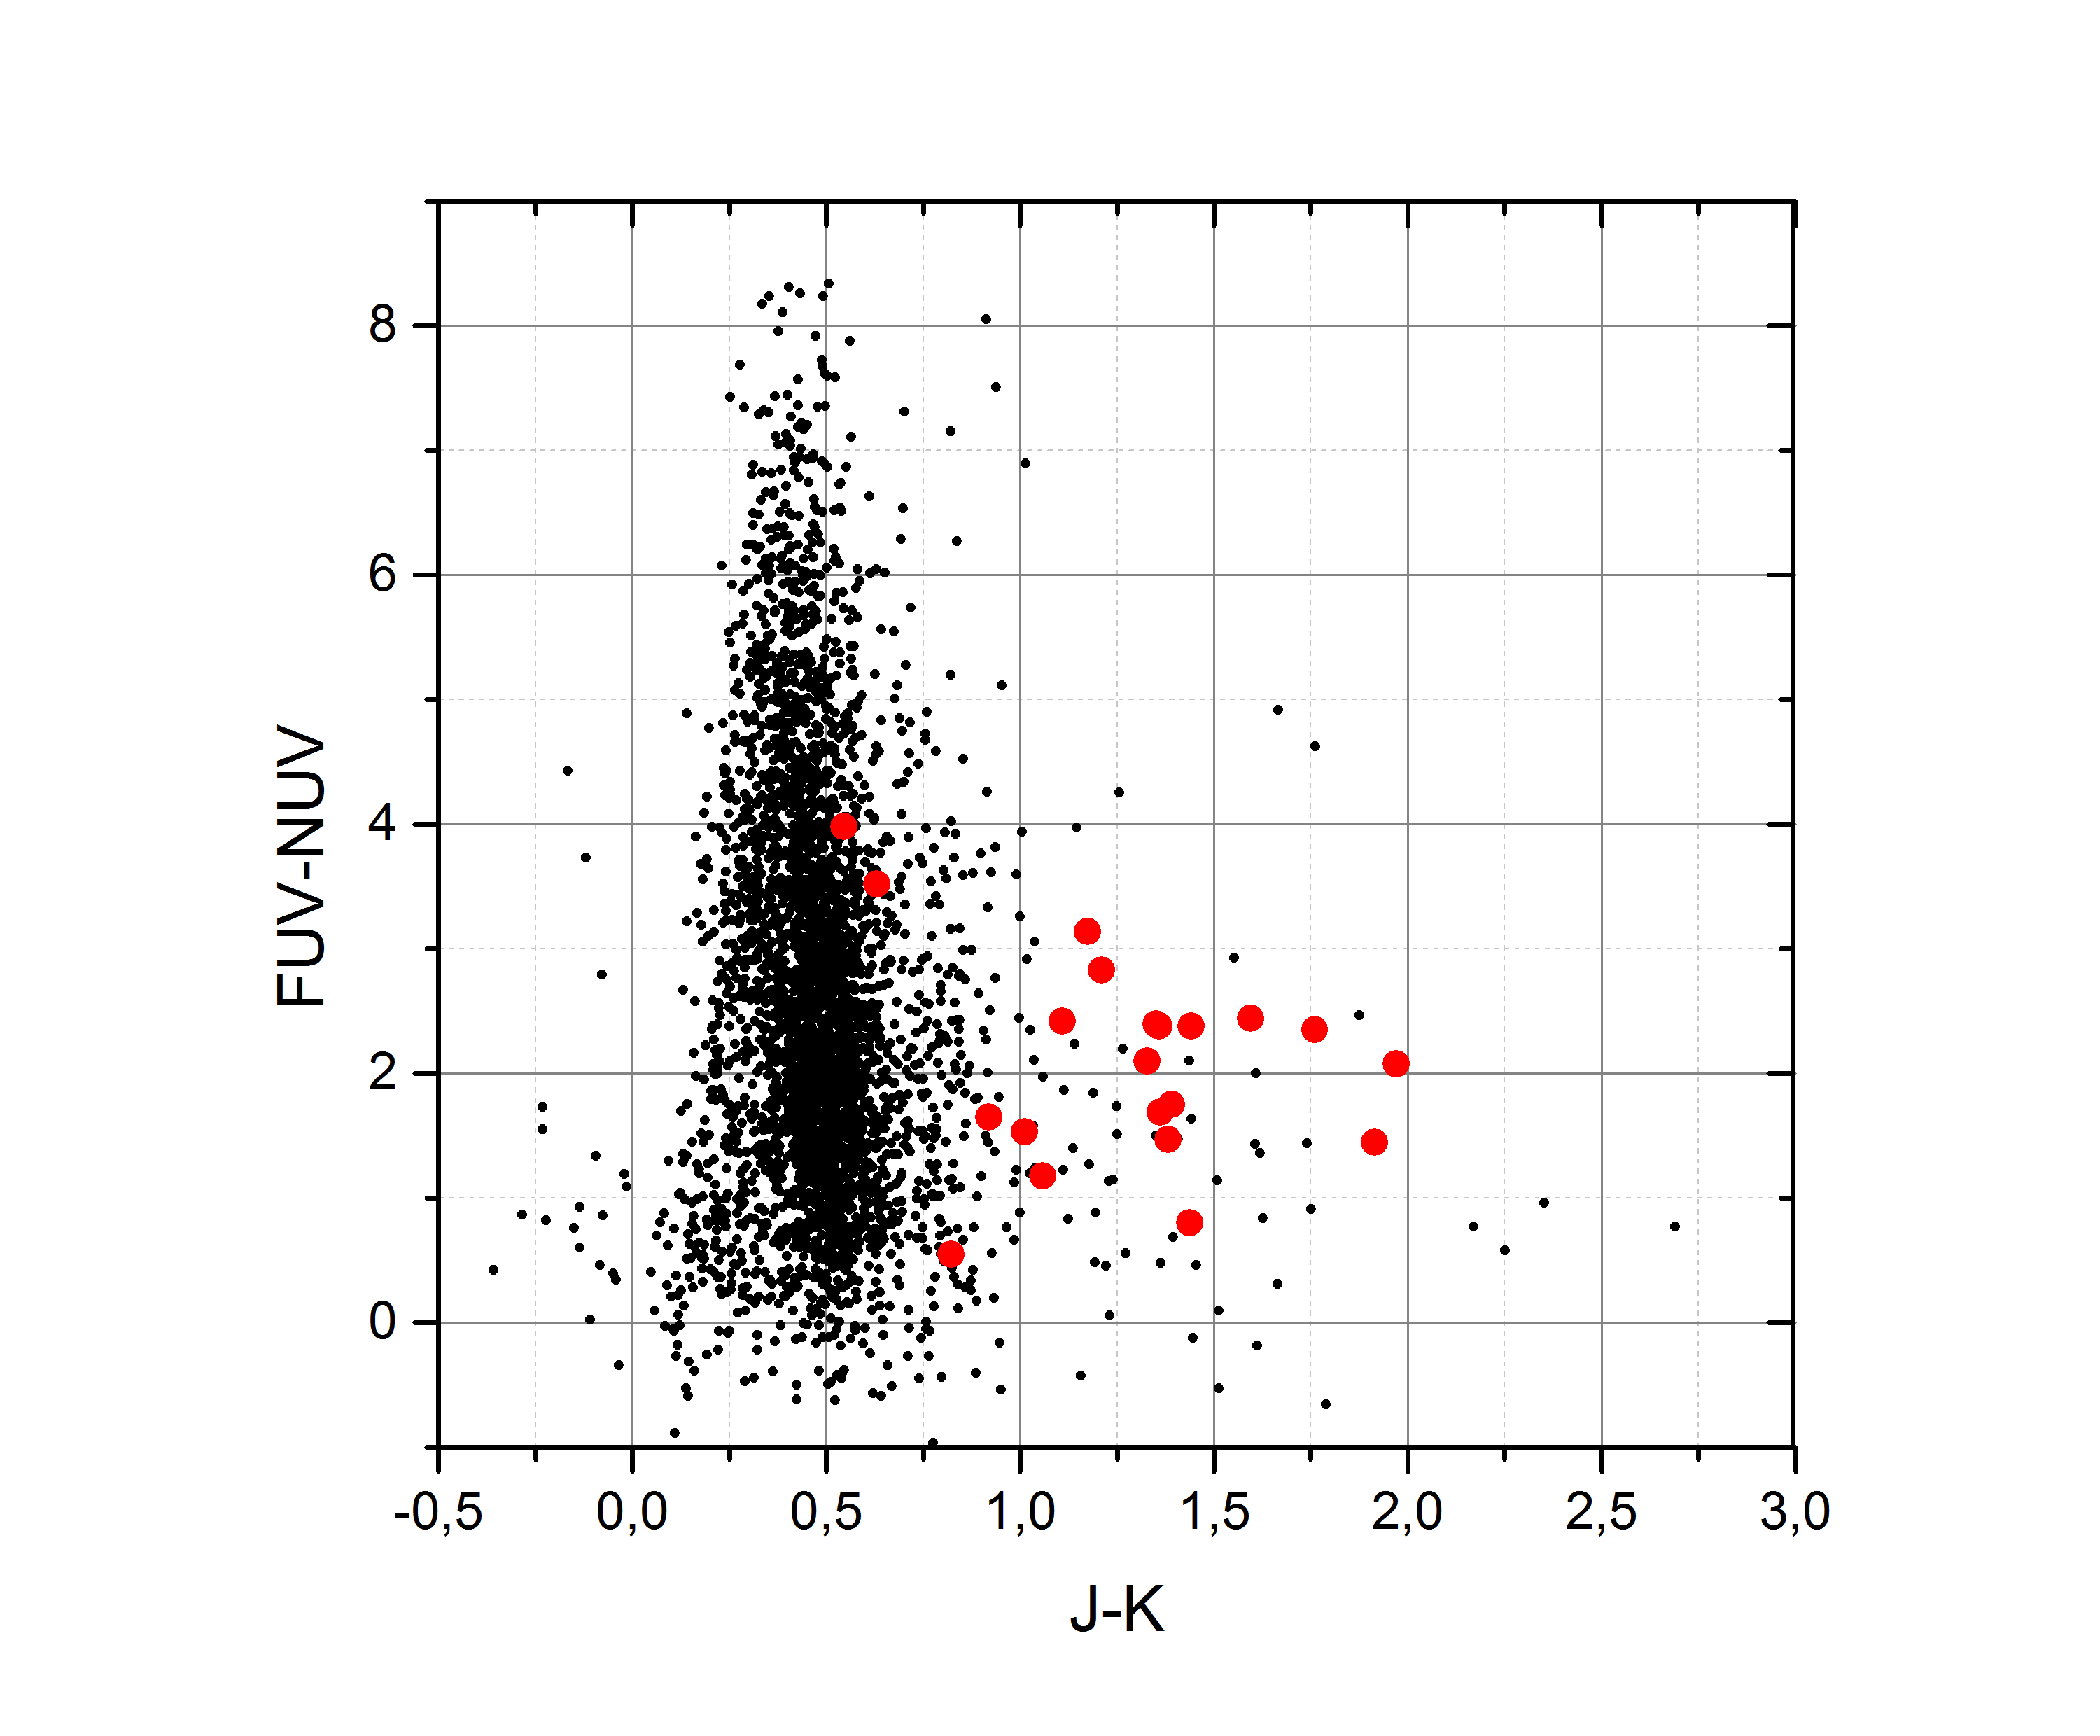
\includegraphics[width=1\linewidth]{Graph1.png} \\ FUV-NUV vs J-K}
\end{minipage}
\hfill
\begin{minipage}[ht]{0.49\linewidth}
\center{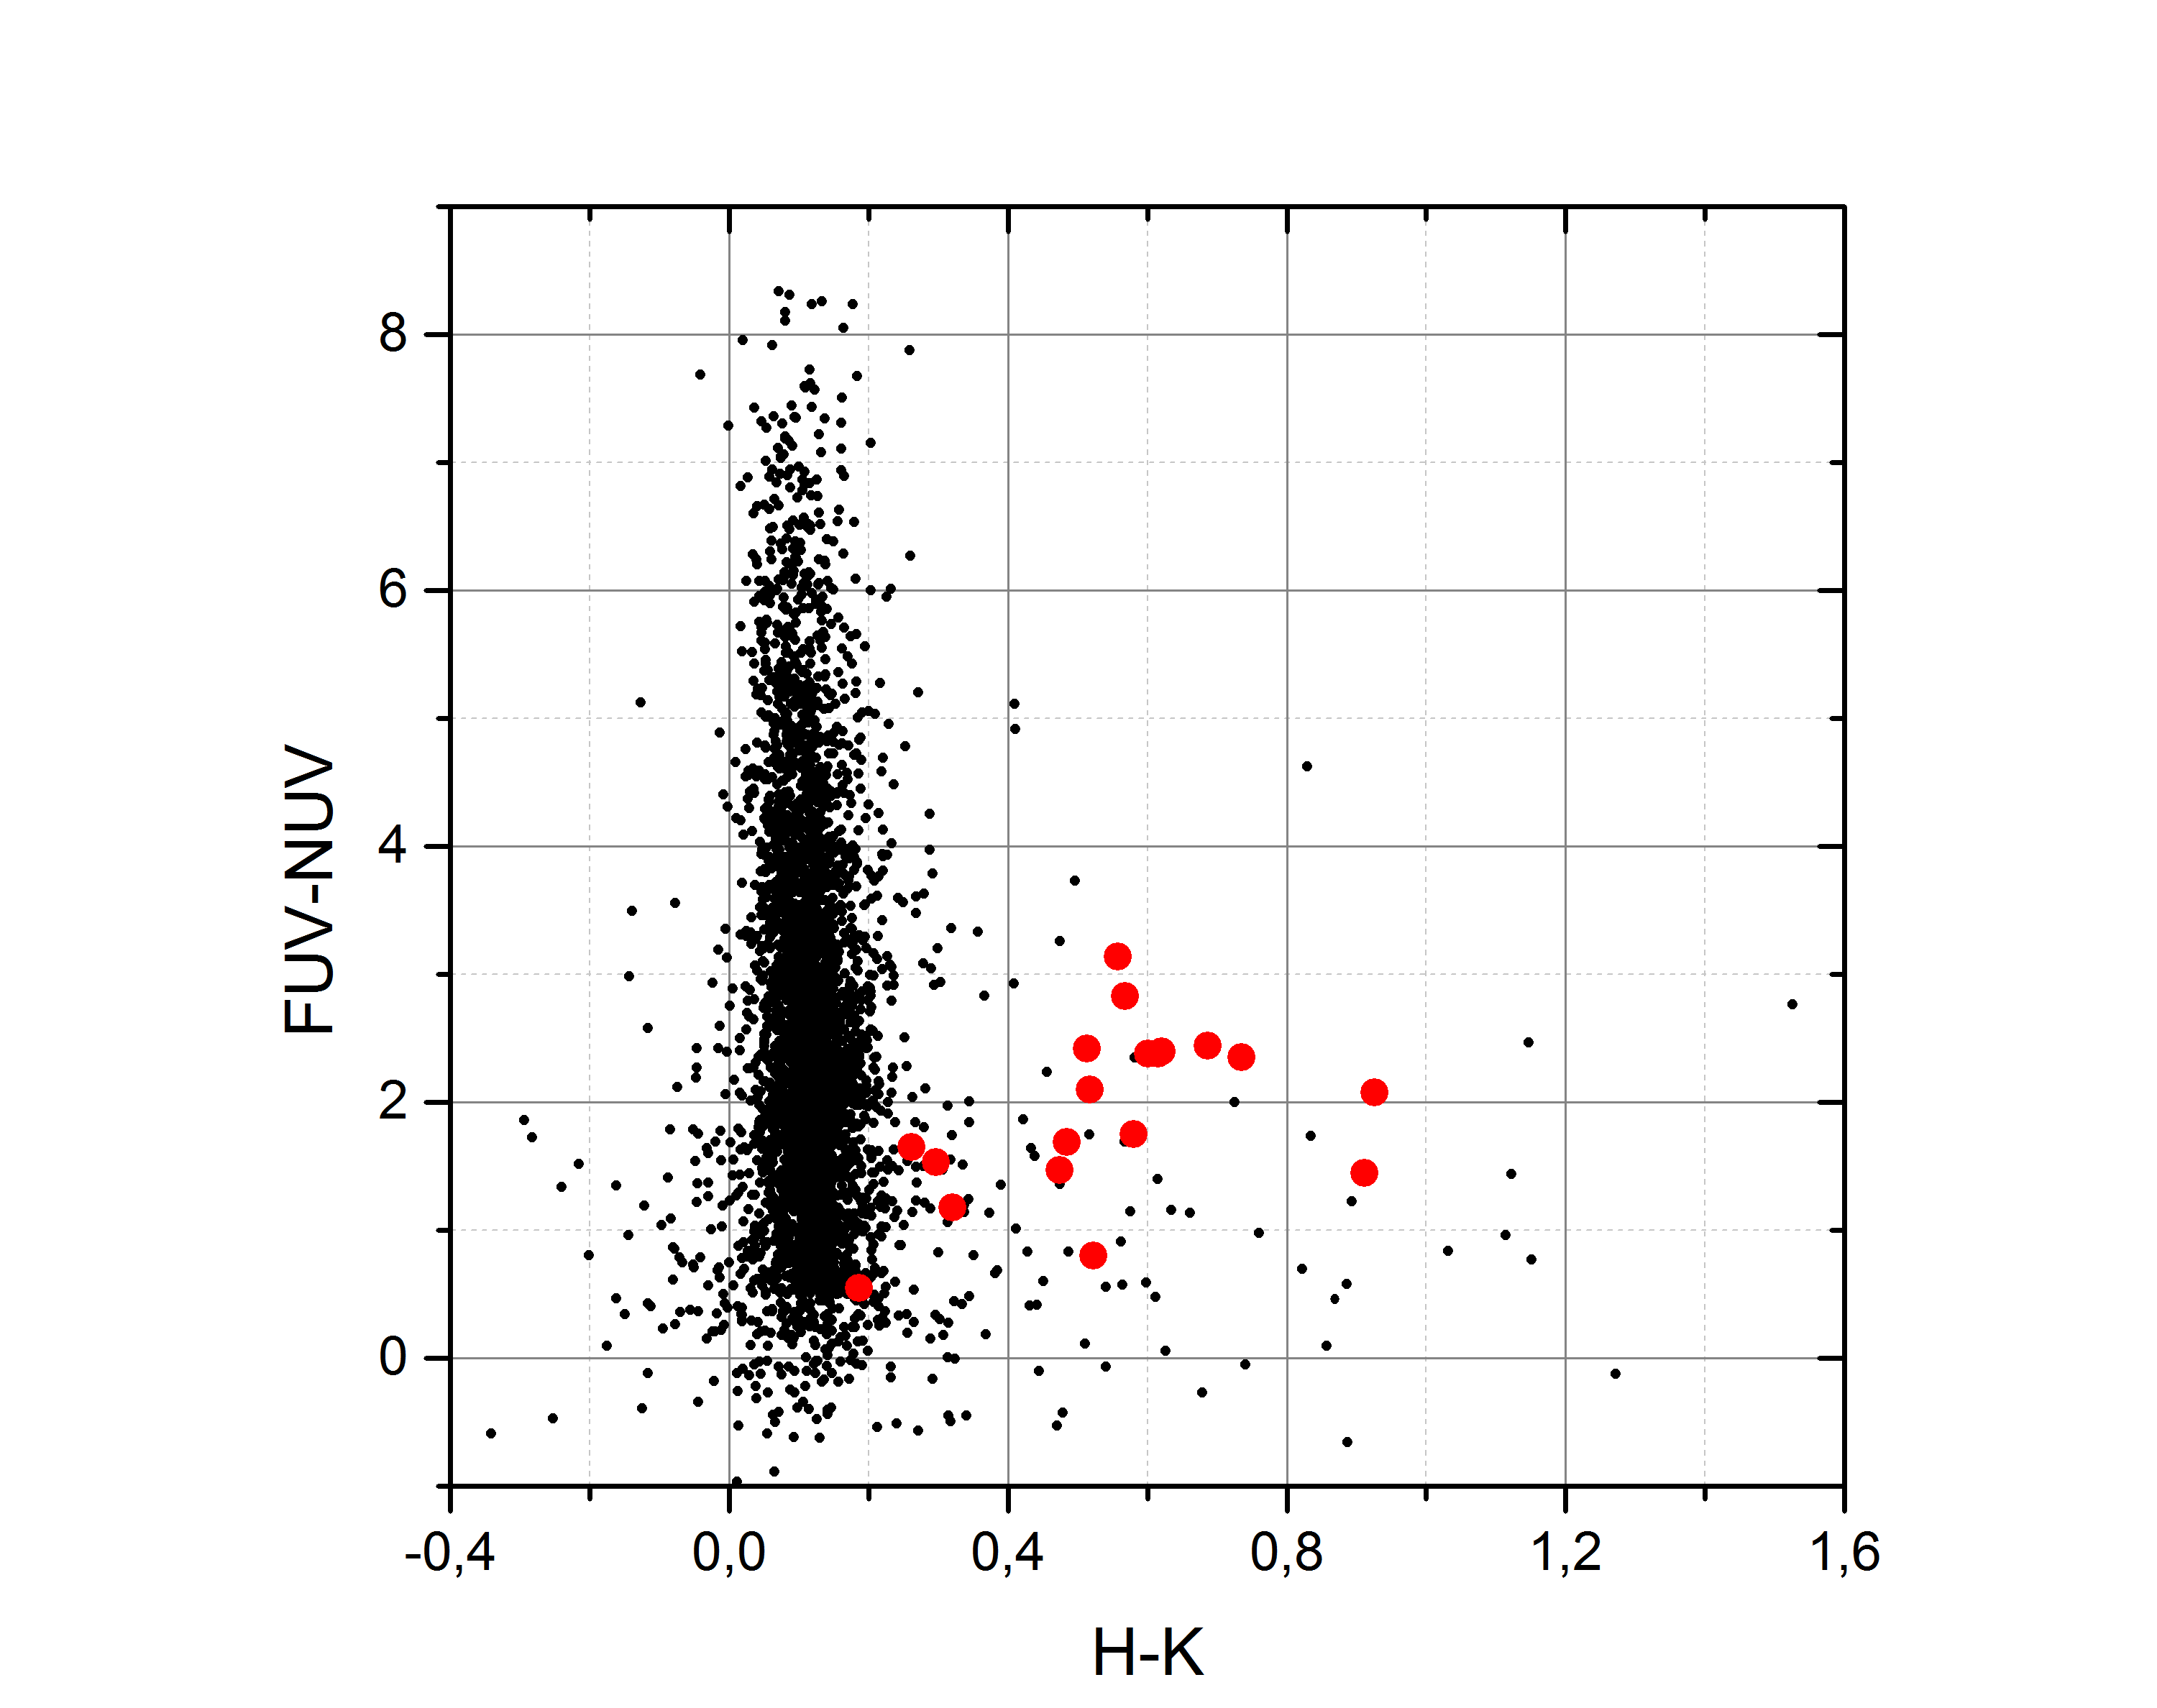
\includegraphics[width=1\linewidth]{Graph2.png} \\ FUV-NUV vs H-K}
\end{minipage}
\begin{minipage}[ht]{0.49\linewidth}
\center{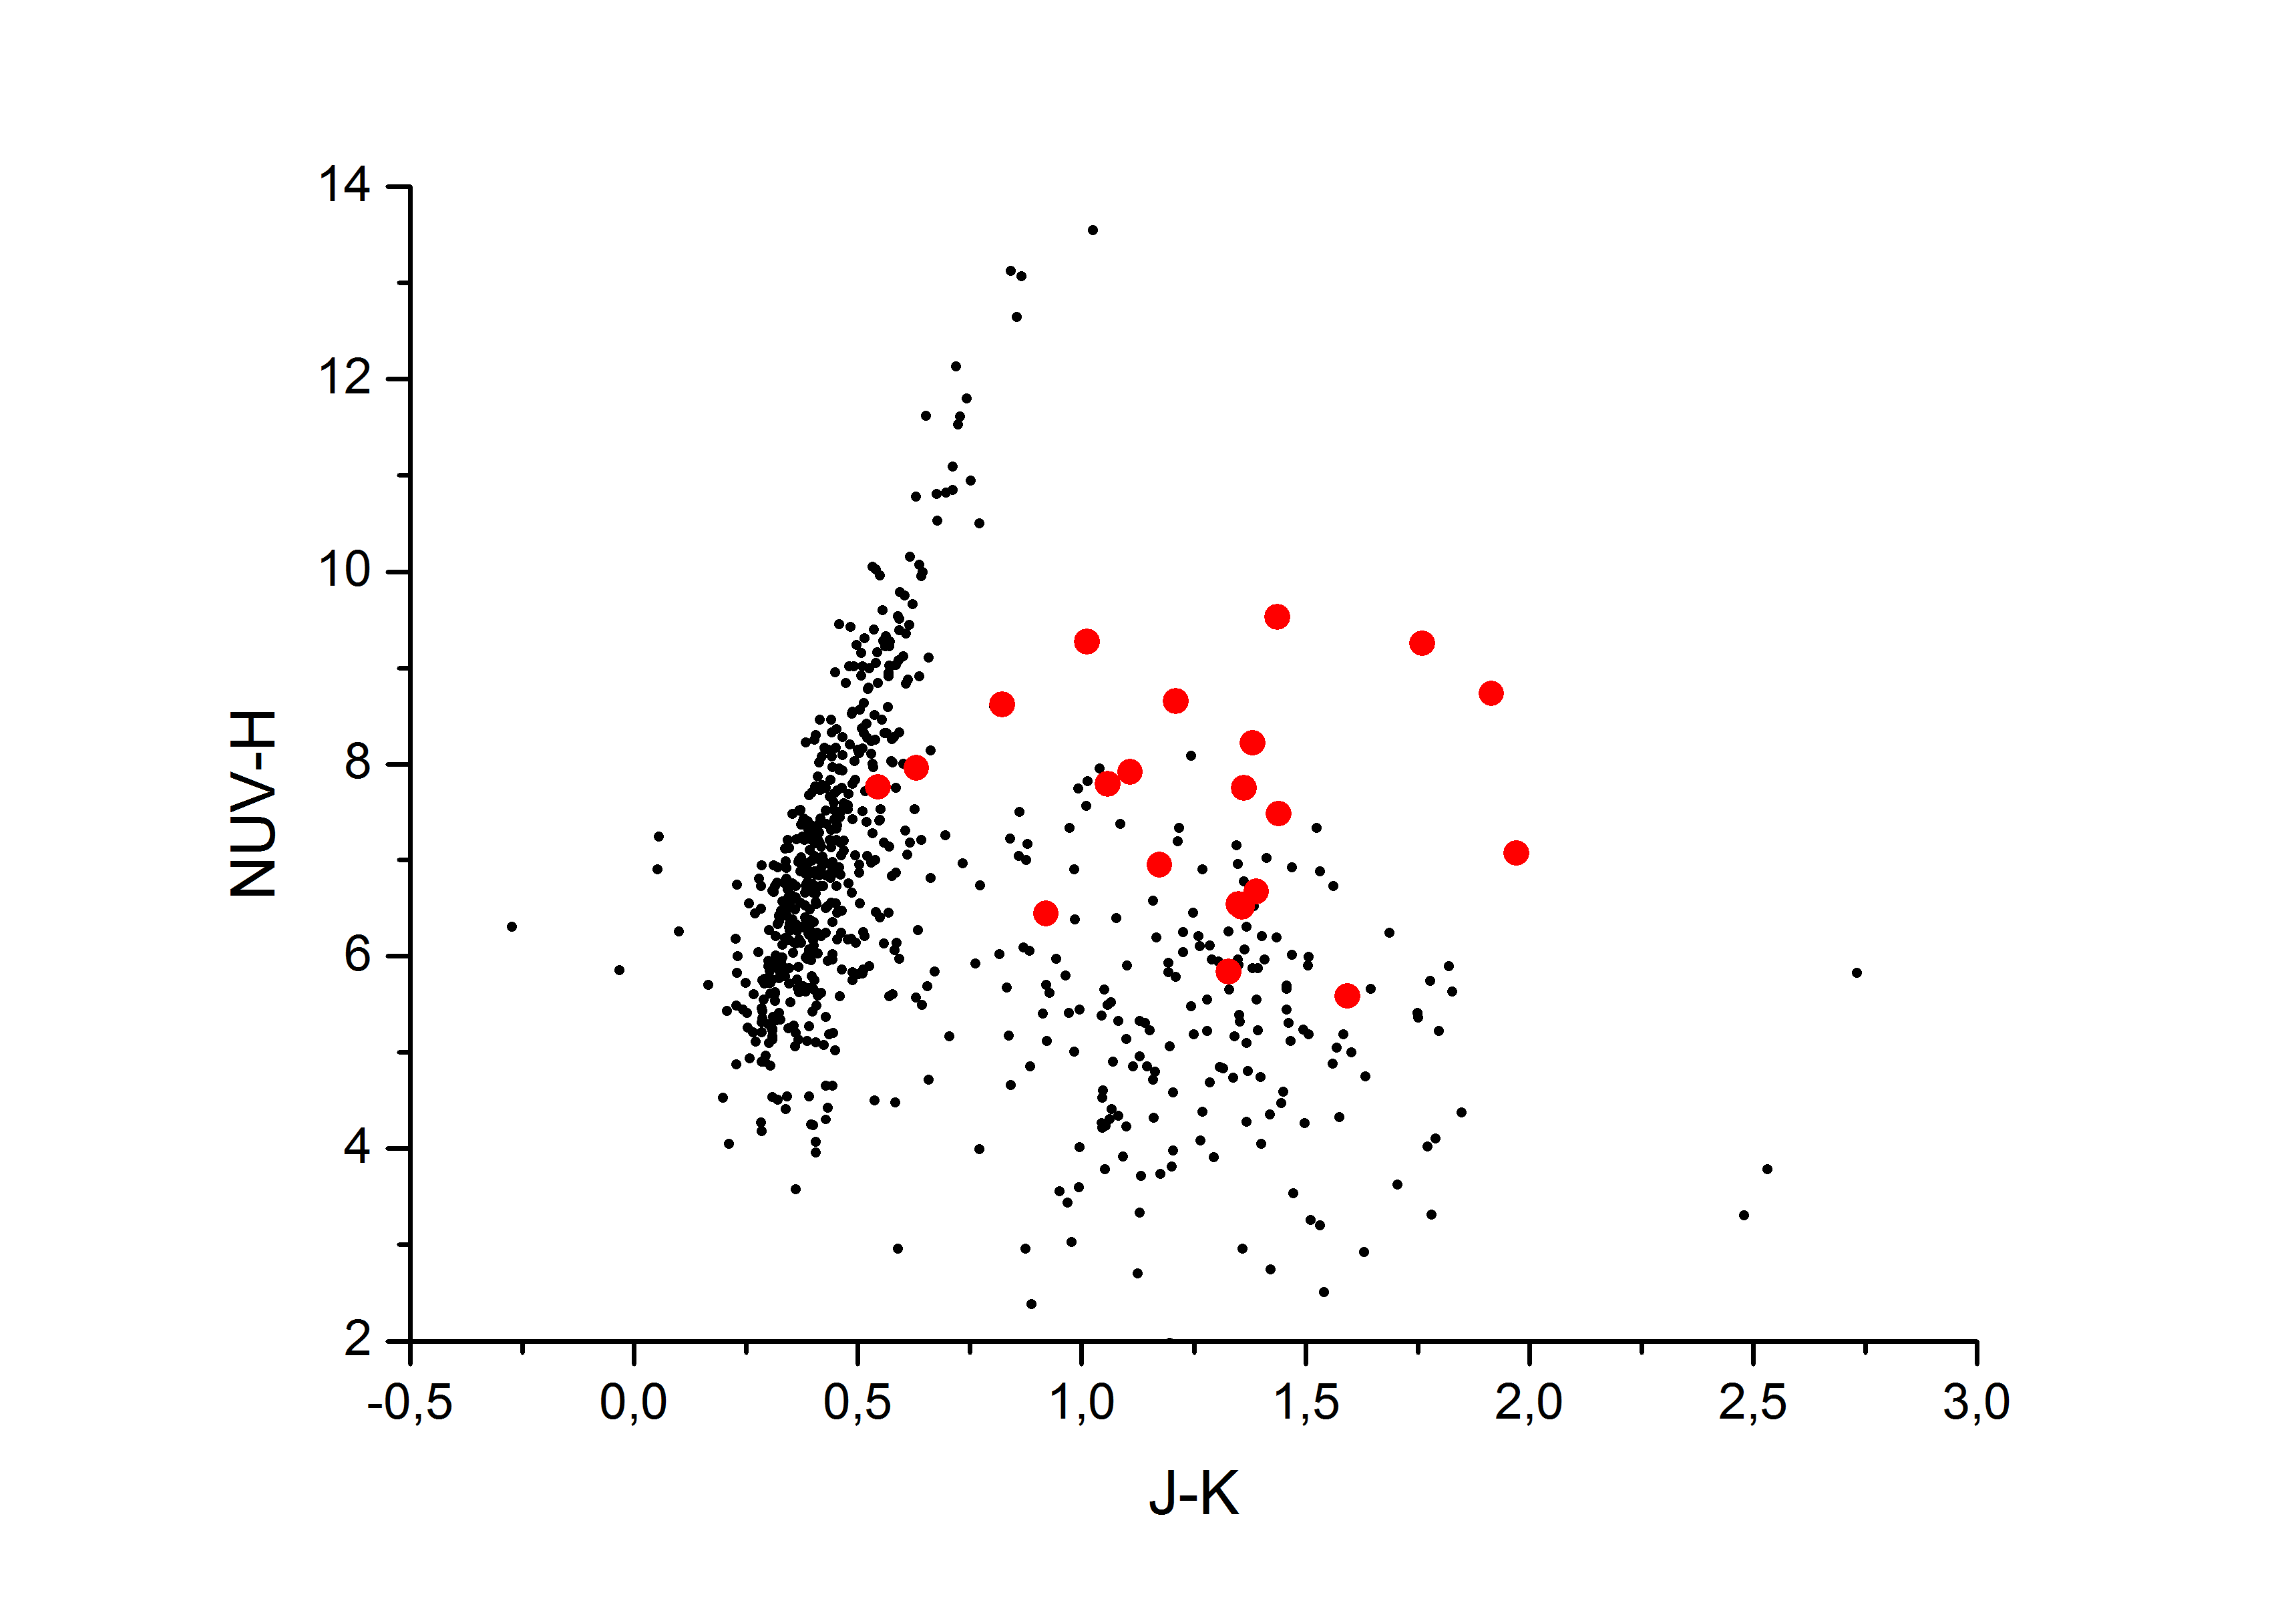
\includegraphics[width=1\linewidth]{Graph3.png} \\ NUV-H vs J-K}
\end{minipage}
\hfill
\begin{minipage}[ht]{0.49\linewidth}
\center{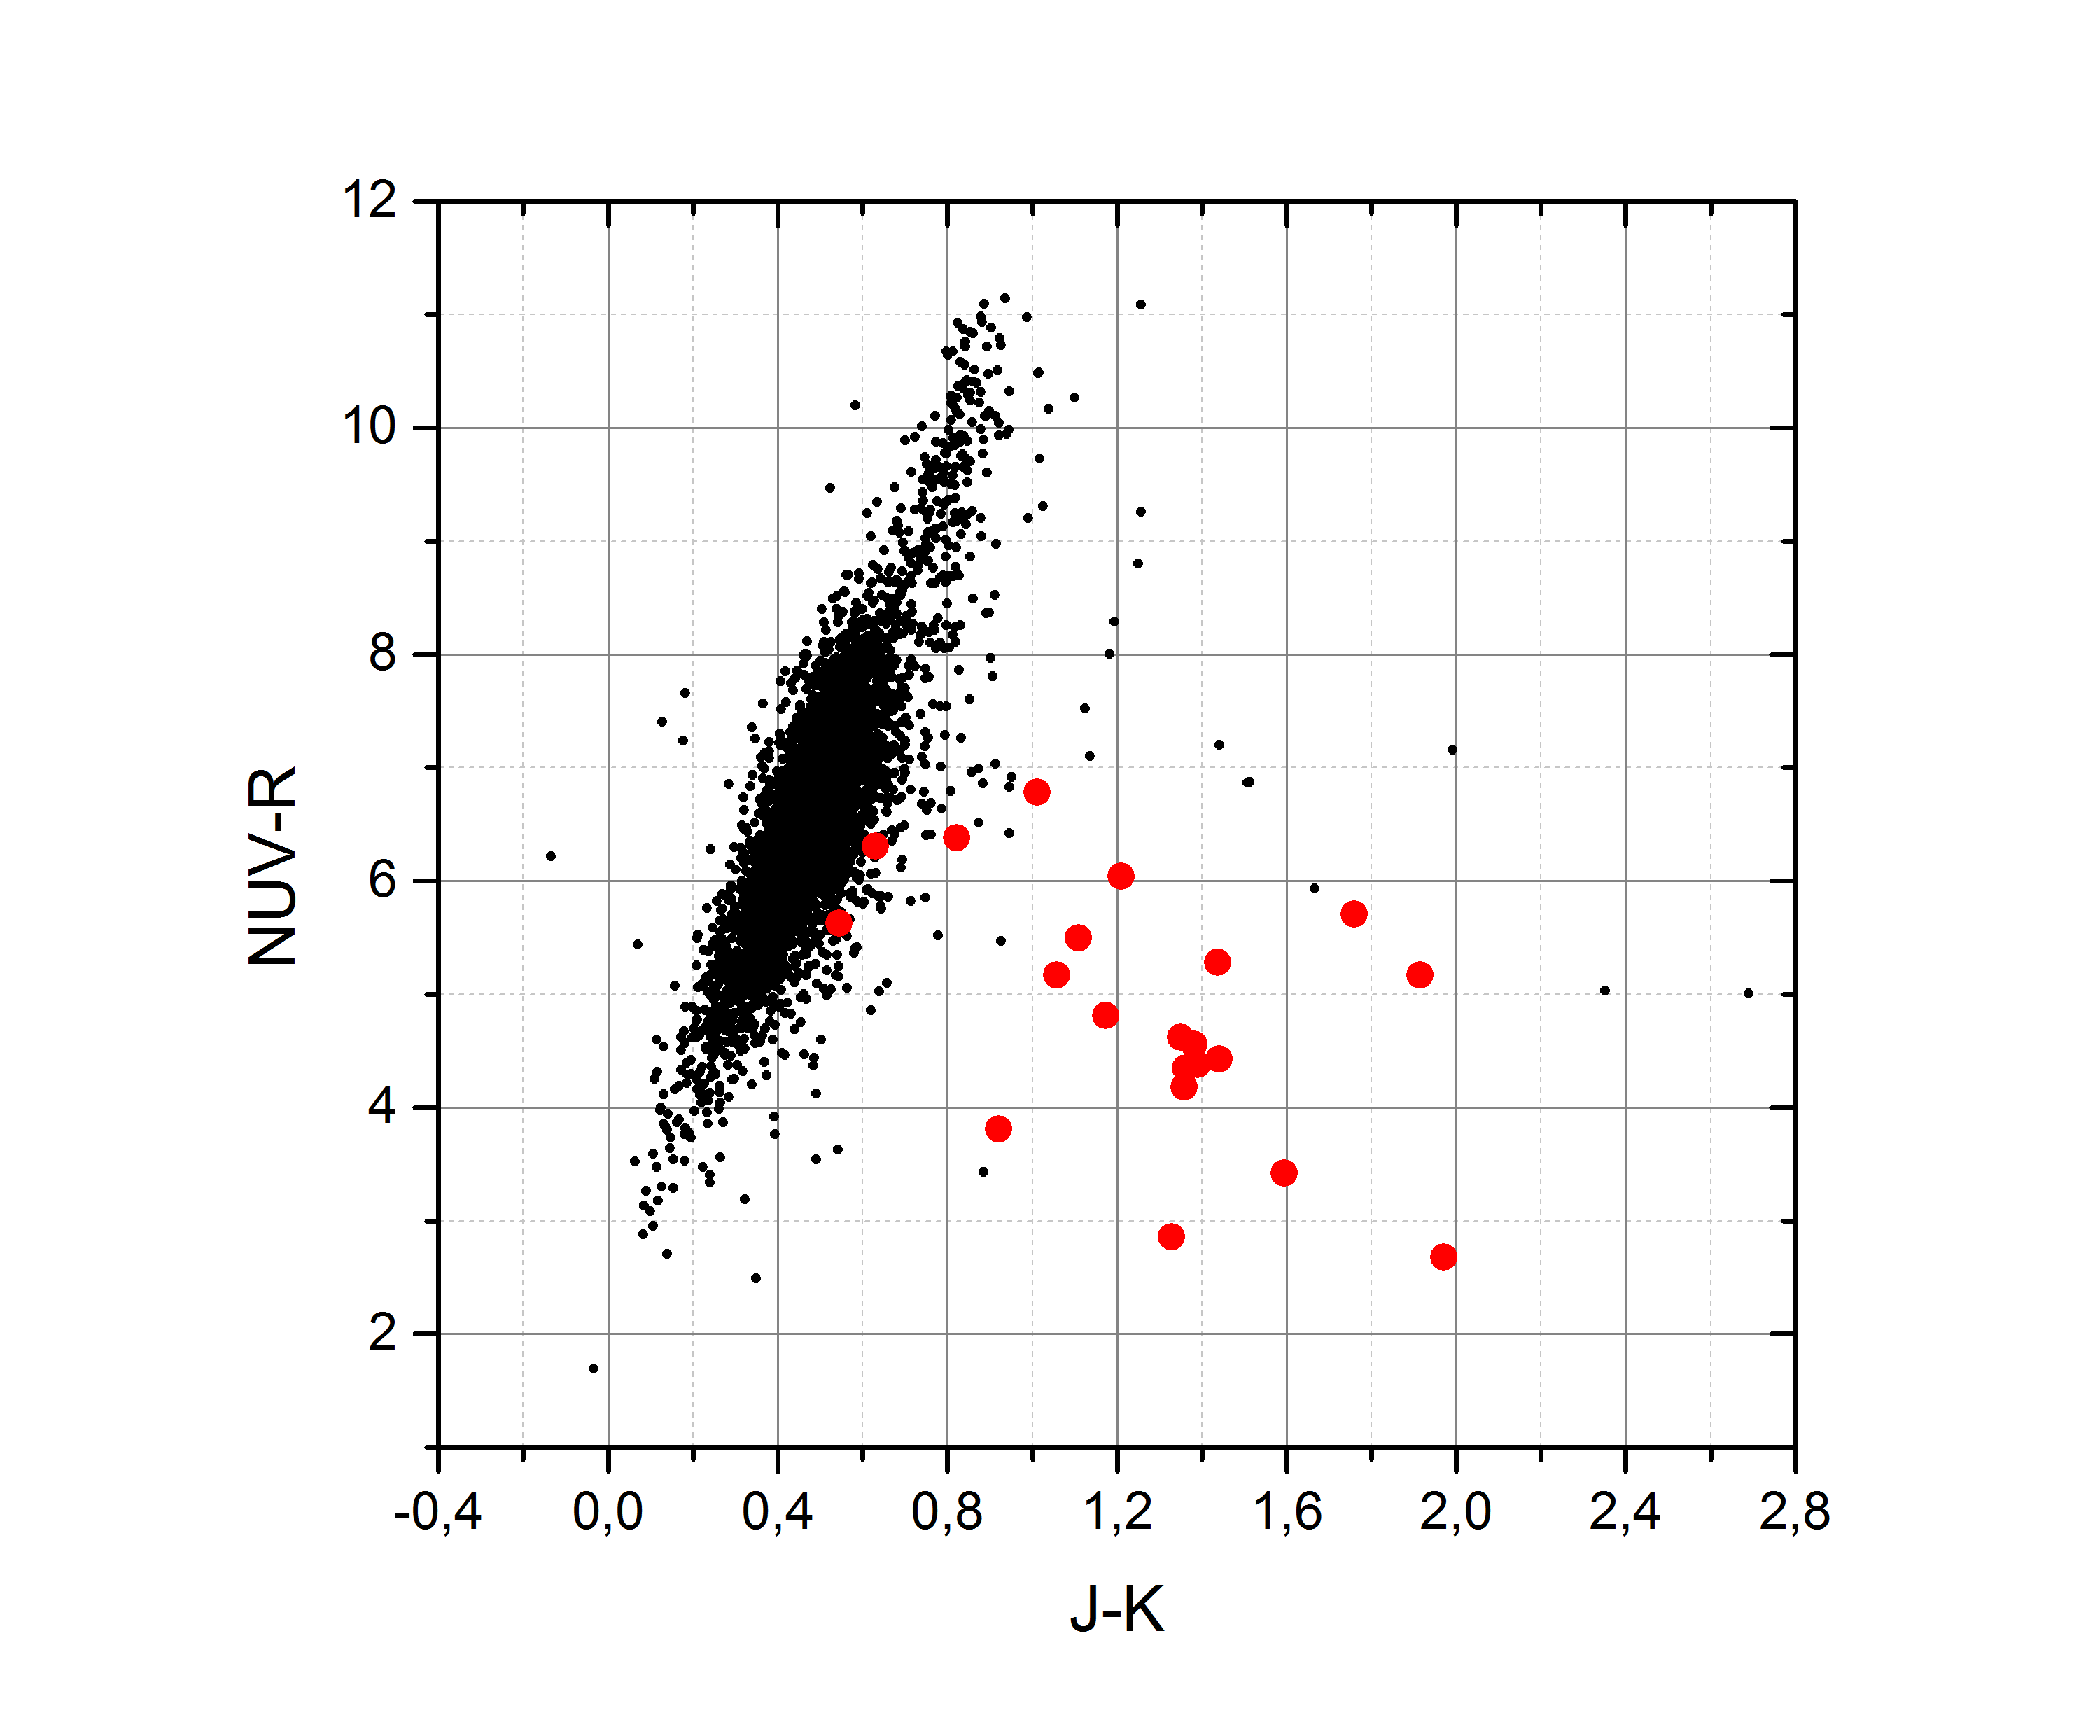
\includegraphics[width=1\linewidth]{Graph4.png} \\ NUV-R vs J-K}
\end{minipage}
\caption{Двухцветные диаграммы. Красным отмечены звёзды эталонной выборки}
\label{fig:colcol}
\end{figure}
Можно объяснить, почему для анализа выбраны именно диаграммы цвет-цвет. Потому что мы не можем сравнивать блеск разных звёзд, он зависит не только от типа звезды, но и от расстояния, поглощения. Нам нужно учесть избыток в инфракрасном диапазоне, поэтому по одной из осей откладывается разность двух ИК звёздных величин. Цвет по другой оси включает УФ величину.

На самом деле в работе \cite{AIGdC2014galex}  приводятся все типы диаграмм, которые мы можем построить, имея исходные данные. Однако именно на выбранных четырёх диаграммах звёзды типа Т Тельца лежат обособленно от остальных, как это видно из положения эталонной выборки.

Звёзды эталонной выборки выделены красным. Заметно, что они группируются в стороне от основной массы звёзд, относящихся к главной последовательности. Также можно видеть, что довольно много звёзд находятся в той же области диаграммы, что и эталоны.

На четвёртом графике рисунка \ref{fig:colcol} рядом с выборкой T Tauri звёзд почти нет других источников. Это связано с тем, что использующийся в данной диаграмме блеск в фильтре R измерен лишь для немногих звёзд в данной области -- тех, что присутствуют в каталоге UCAC4. 

\section{Критерии отбора}

В выборку включим все звёзды, положение которых на диаграммах близко к положению известных T Tauri. Для этого зададим границы, в которые должны входить цвета, причём все эталонные звёзды также должны попадать в эти границы.

На диаграмме NUV-H vs J-K эталонные T Tauri особенно сильно отделены от остальных звёзд. Это обусловлено тем, что в выборку IUE входят в основном яркие звёзды. К тому же большинство из них находится ближе, и как следствие меньше подвержено поглощению. Ниже группы эталонных звёзд на этой диаграмме находится много точек, у которых NUV-H меньше. Предполагая, что эти источники подверглись большему поглощению, то есть находятся глубже в молекулярном облаке, мы также включим их в список кандидатов, сдвинув границы по NUV-H в нижнюю сторону.

Диаграмма NUV-R от J-K должна дать нам не очень много кандидатов, однако её тоже нужно учесть. Как и NUV-H vs J-K, она даёт шанс неярким звёздам с неизмеренным FUV попасть в список кандидатов.

Теперь мы можем сформулировать критерии первичного отбора кандидатов:
\begin{itemize}
	\item FUV-NUV vs J-K: звёзды типа Т Тельца должны удовлетворять 0.5 < J - K < 2.4 и 0.4 < FUV - NUV < 4.6;
	\item	FUV-NUV vs H-K: звёзды типа Т Тельца должны удовлетворять 0.2 < H - K < 1.2 и 0.4 < FUV - NUV < 4.6;
	\item	NUV-H vs J-K: звёзды типа Т Тельца должны удовлетворять 0.5 < J - K < 2.4 и 4.2 < NUV - H < 11.0;
	\item	NUV-R vs J-K: звёзды типа Т Тельца должны удовлетворять 0.5 < J - K < 2.4 и 1.5 < NUV - R < 8.2;
\end{itemize}

Наша цель -- не только найти кандидаты в T Tauri звёзды, мы хотим, чтобы ни одна из них не была потеряна в ходе отбора, если это возможно. Поэтому на этом этапе мы оставляем те источники, которые удовлетворяют хотя бы одному из четырёх критериев.

Первые два критерия -- основные. Звёздные величины и цвета, входящие в них, соответствуют спектральным особенностям T Tauri звёзд, отличающих их от звёзд главной последовательности. Третий и четвёртый критерий тоже учитывают ультрафиолетовый избыток, так как в фильтр NUV попадают многие ключевые линии: (такие-то). Однако они подходят и для более слабых звёзд: тех, что находятся глубже в молекулярном облаке, чьё более коротковолновое излучение не дошло до нас из-за поглощения; для звёзд типа Т Тельца со слабыми линиями, у которых избыток настолько слаб, что не был зафиксирован детекторами GALEX.

\section{Результат и адекватность критериев}
После применения этих критериев к исходному списку мы получили следующие результаты.

Первому критерию удовлетворяет 164 источника, второму -- 100 источников, третьему -- 274, и четвёртому 94. В общий в список, включающий объединение этих четырёх, попало 302 источника.

Следует отметить, что последний критерий не добавляет ни одного нового источника в итоговый список, то есть нет кандидатов, удовлетворяющих одному лишь четвёртому критерию. Первые два критерия (основные) в сумме дают 215 источников. Оставшиеся 87 кандидатов попали в список по третьему критерию. Они могут не иметь FUV блеска.

Эффективность этих критериев может быть проверена по их способности детектировать все известные в изучаемой области звёзды типа Т Тельца. Но в туманности в созвездии Змея нет ни одной звезды, классифицированной как T Tauri, и ни одной, классифицированной как кандидат в T Tauri звёзды. Поэтому мы не можем проверить это напрямую.

Однако в работе \cite{AIGdC2014galex}, в которой аналогичные критерии применялись к звёздам в молекулярном облаке Тельца, эффективность критериев была проверена. Они оказались способны обнаружить все известные в TMC T Tauri звёзды, которых там насчитывается 31. 

Желание не упустить ни одну известную  звезду является одной из причин выбора более широких границ цвета при составлении критериев.

